% !TEX root = ./chemistry.tex

\chapter{Module 7 - Organic Chemistry}

\section{Hydrocarbons} \label{02/05/2025}

	\subsection{Bonding in Carbon}
	
		Carbon atoms almost always form four covalent ($\because$ non-metal) bonds because of it's valency of 4.

		In alkanes (single bond compounds)

		One, two or three pairs of the valence electrons from adjoining carbon atoms may be involved in the bonding to form :

			\begin{itemize}
				\item single bonds \ce{C-C}
				\item double bonds \ce{C=C}
				\item triple bonds \ce{C#C}
			\end{itemize}

		When four carbon atoms bond to each other, a different type of substance forms. This is due to the varying structures in each type of covalent network lattice. Each structure is called an \textbf{allotrope}

	\begin{figure}[H]
		\centering
		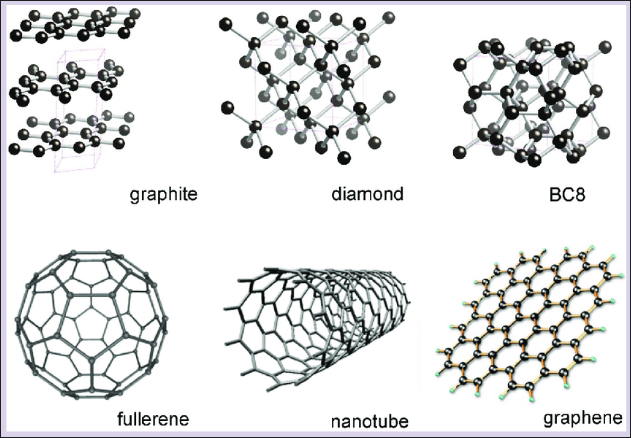
\includegraphics[width=8cm]{covalent_carbon_structure.png}
	\end{figure}

	\subsection{Types of Hydrocarbons}
	
		Hydrocarbons are compounds made up of only hydrogen and carbon

		\textbf{Aromatic} hydrocarbons contain one or more benzene rings

		\textbf{Aliphatic} compounds are all the other hydrocarbons. The carbon atoms may be bonded in chains or non-aromatic rings. The chain of compounds may be further classified into families on the basis of individual carbon-carbon bonds.

	
	\subsection{Aliphatic Hydrocarbons}
	
		\begin{enumerate}
			\item If all carbon-carbon bonds are single bonds, the compound is an \textbf{alkane}. These are called \textbf{saturated compounds}.
			\item Compounds in which at least one of the carbon-carbon bonds is a double bond are called \textbf{alkenes}. Compounds with at least one multiple bond are called \textbf{unsaturated compounds}.
			\item Alkynes have at least one carbon-carbon triple bond. They are classified as unsaturated compounds.
			\item Hydrocarbon compounds in which the carbon atoms have joined to form a closed ring structure are called \textbf{alicyclic}, or more commonly, cyclic hydrocarbons.
		\end{enumerate}

	\subsection{Representing Organic Molecules}
	
		A \textbf{molecular formula} such as \ce{C3H8} gives information on the number of atoms, but nothing about the arrangement of those atoms.

\textbf{Structural formulae} are used to represent organic molecules as the arrangement of atoms can vary greatly within molecules with the same molecular formula.

	\subsection{Check Your Understanding - 8.1}
	
		\begin{enumerate}
			\item \textbf{Describe how the valence electrons of carbon are involved in bonding in organic compounds}
				\subitem The four valence electrons in the carbon atom allow it to form four covalent bonds with other atoms

			\item \textbf{Describe the differences between:}
				\begin{enumerate}
					\item aromatic and aliphatic compounds - aromatic compounds contain a benzene ring whereas aliphatic do not
					\item saturated and unsaturated compounds - saturated only single, unsaturated have varying
				\end{enumerate}
		\end{enumerate}

\section{Alkanes}

	Alkanes are important because it includes the fuels that supply energy

	Light gases have small molecules with:

	\begin{itemize}
		\item Low boiling point
		\item Light in colour
		\item Easy to light
		\item Runny
	\end{itemize}

	Including methane, ethane, propane, and butane

	Longer chained hydrocarbons have a higher boiling point. When boiling, intermolecular forces are broken (which are dispersion forces in hydrocarbons). The longer the chains, the more hydrogen is present, making it harder to separate each molecule apart.

		\subitem 1 - meth

		\subitem 2 - eth

		\subitem 3 - prop

		\subitem 4 - but

		\subitem 5 - pent

		\subitem 6 - hex

		\subitem 7 - hept
		
		\subitem 8 - oct
		
		\subitem 9 - non

		\subitem 10 - dec

	The alkanes are known as a homologous series; a group of compounds with the same general formula.
	
	\subsection{Rules for Naming Alkanes}
	
		\begin{enumerate}
			\item The end of the name indicates which hydrocarbon family the compound belongs in. Alkanes end in -ane.
			\item Determine the longest continuous carbon chain and use the name of the corresponding alkane. This is the \textbf{main chain}.
			\item Other atoms of groups of atoms attached to the main chain are called substituents and form "branches". If the substituent is a carbon group, then it is called an alkyl group. Alkyl groups are given the ending -yl.
			\item Number the carbons in the main chain so the branch of branches have the lowest possible numbers.
			\item The position at which the group is attached to the main chain is specified by the number of the carbon to which it is attached. The number is separated by a hyphen.
			\item The names of the substituents are given in \textbf{alphabetical order}.
		\end{enumerate}

\section{Alkenes} \label{07/05/2025}
	
	The alkene family contains hydrocarbons in which one pair of carbon atoms is joined by a double bond, and all other carbons are joined by single bonds. This double bond means that the hydrocarbon is unsaturated.

	Alkenes have the general formula \ce{C_{n}H_{2n}}

	\subsection{Naming Alkenes}

		The process of naming alkenes is similar to that of alkanes, however the position of the double bond can change.

		\begin{enumerate}
			\item Take the usual stem name (eg. eth-, bu-) and add the suffix -ene.
			\item Show the location of the double bond by numbering the carbon atoms from the end of the chain closest to the double bond; ie. get the smallest number, eg. a 1-butene hydrocarbon would have a double bond between the 1 and 2 carbon atoms
			\item Branched alkenes have the same rules as branched alkanes
			\item The double bond is prioritised over substituents when determining the end of the hydrocarbon to start at
		\end{enumerate}

\section{Alkynes} \label{08/05/2025}

	Alkynes are a family of hydrocarbons containing at least one triple bond between a pair of carbon atoms. Like the alkenes, alkynes are unsaturated.

	Alkynes have a general form of \ce{C_{n}H_{2n-2}}

	The naming process is identical to that of alkenes

\section{Halogenated Organic Compounds}

	Organic compounds that contain one of more halogen atoms (bromine, chlorine, fluorine, or iodine) attached to one of the carbon atoms in the molecule.

	\subsection{Naming Hydrocarbons with Halogen Atoms}
	
		\begin{enumerate}
			\item Name the parent chain as normal
			\item Alkyl side chains are identified and named as normal
			\item Any halogen atoms are identified with the place number of the carbon they are attached to. Their name is given as follows:
				\begin{itemize}
					\item fluorine $\rightarrow$ -fluoro
					\item chlorine $\rightarrow$ -chloro
					\item bromine $\rightarrow$ -bromo
					\item iodine $\rightarrow$ -iodo
				\end{itemize}
			\item All branches are listed in alphabetical order
		\end{enumerate}

\section{Isomers}

	Compounds that have the same molecular formula but different structural formula are called structural isomers.

	In hydrocarbons, isomers can occur by changing the position of double or triple bonds, or different placement of substituents (positional isomers).

	Chain isomers involve rearrangement of the carbon skeleton.

\section{Benzene}

	An unsaturated aromatic compound with delocalised electrons with formula \ce{C6H6}. It has a shape of a flat hexagon

	Benzene rings have carbon bonds of the same length, however the length of the each bond lies between a single bond and a double bond. The double bonds are not drawn because they can exist either in place 1, 3, 5 or 2, 4, 6 with each structure being structurally equivalent. A circle is drawn in the centre to represent the electron cloud.
	
	\begin{center}
		\chemfig{C*6((-H)-C(-H)=C(-H)-C(-H)=C(-H)-C(-H)=)}
	\end{center}

	The cyclic delocalisation of electron makes it extremely stable

\section{Properties of Alkanes}

	Alkanes are covalent molecular substances so they will have similar physical properties to other covalent molecules.

	Carbon and hydrogen have similar electronegativity and most hydrocarbons are relatively symmetrical, making them non-polar.

	Alkenes and alkynes have a similar structure to alkanes, and so share the same physical properties.

	Alkanes have relatively low melting and boiling points since dispersion forces are the only type of intermolecular force that forms between molecules. As the size of the molecule increases, more atoms are present, increasing the number of electrons in the molecule. Thus the strength of the overall dispersion forces between molecules increases.

	Larger molecules require more energy to overcome the dispersion forces, hence \textbf{Longer carbon changes have higher melting and boiling points}

	For example, shorter chain alkanes like ethane and propane are gases at room temperature in comparison to octane and oils being liquids and very long chains like wax and tar being solids.

	The shape of the hydrocarbon also changes the boiling and melting points of a compound. Linear molecules pack closely and allow many dispersion forces to form, creating a greater attraction between molecules. Bulky molecules no not neatly pack together, therefore have smaller boiling and melting points.

	Lack of polarity means that hydrocarbons are not conductive or soluble in water

\section{Uses of Alkanes}

	\begin{itemize}
		\item Methane is a main component of natural gas
		\item Propane is also known as liquid petroleum gas (LPG)
		\item Pentane is used as an industrial solvent
		\item Octane is the main constituent of automobile fuel
		\item Nonane and decane are used in petrol as additives
	\end{itemize}

\section{Uses of Alkenes}

	\begin{itemize}
		\item Basis of petrochemical industry, especially those with low molecular mass
		\item Used as starting materials in the syntheses of alcohols, plastics, lacquers, detergents, and fuels
		\item Ethene is the most important organic feedstock in the chemical industry. A feedstock is a chemical or substance that is used to manufacture useful materials and other chemicals
		\item Used for making polyethylene, vinyl chloride, styene, artificial ripening of fruits, general anaesthetic
	\end{itemize}

\section{Functional Groups}

	A group or family of organic properties. Substances within a particular family containt a specific atom or group of atoms called a functional group.

	\begin{table}[H]
		\centering
		\setstretch{1.25}
		\begin{tabular}{l|l|l}
			Class & Suffix & Functional Group \\ \hline
			Haloalkane & -ane & -F, -C, -Br, -I \\
			Alcohol & -ol & -OH \\
			Aldehyde & -al & -C=O,-H \\
			Ketone & -one & \\
			Carboxylic acid & -oic acid & \\
			Ester & alkyl -oate & \\
			Amine & -amine & \\
			Amide & -amide &
		\end{tabular}
	\end{table}

\section{Alcohols}


	\subsection{Naming Alcohols}
	
		\begin{enumerate}
			\item Identify the longest carbon chain
			\item Write the alkane name without the "e" at the end and replace it with "ol"
			\item Similar to identifying the position of the double bond in alkenes, the position of the \ce{-OH} group is identified by using a number in front of the main alcohol name
		\end{enumerate}

	\subsection{Types of Alcohols}
		
		Alcohols can be classified according to the number of carbon atoms attached to the carbon bearing the \ce{-OH} group.

		Primary: butan-1-ol

		\begin{center}
			\chemfig{CH_3-CH_2-CH_2-CH_2-OH}
		\end{center}

		Secondary: butan-2-ol

		\begin{center}
			\chemfig{CH_3-CH_2(-[2]CH_3)-CH_2-CH_3}
		\end{center}

	\subsection{Properties of Alcohols}
	
		The hydroxyl group in alcohols contains a highly electronegative oxygen atom, thus making a highly polar \ce{C-O} and \ce{O-H} bond.

		The properties of alcohols depend on the presence of the \ce{-OH} group and the size of teh hydrocarbon chain.

		The boiling point of an organic compound relates to the energy required to overcome intermolecular forces between molecules.

		Hydrogen bonding in alcohols is stronger than dispersion forces, therefore it will have a significantly higher boiling point than alkanes of similar molecular mass.

	\subsection{Solubility}
	
		Alcohols with a smaller hydrocarbon chain are very soluble in water. The polar \ce{-OH} group forms hydrogen bonds with water, making short chains soluble. The non-polar hydrocarbon chain cannot form hydrogen bonds so is not soluble. As the length of the hydrocarbon chain increases, the solubility decreases.

		An example of a large molecule with high solubility in water is glucose, \ce{C6H12O6}

\section{Aldehydes and Ketones} \label{12/05/2025}

	Carbonyl compounds are those double bonded to an oxygen atom. Both aldehyde and ketones are carbonyl compounds.

	Aldehydes are carbon compounds that contain a carbon-oxygen double bond at the end of the carbon chain. The compound is represented by the general molecular formula:

	\begin{center}
		\chemfig{R-{CH}(=[2]O)}
	\end{center}

	Methanal (\ce{HHCO}), commonly known as formaldehyde is the simplest aldehyde. Methanal is used in vast quantities in the manufacture of plastics.

	Ketones differ from aldehydes in that the \ce{C=O} can be located on any carbon except those at the ends of the hydrocarbon chain. The compounds have the general formula:

	\begin{center}
		\chemfig{R-C(=[2]O)-R'}
	\end{center}

	Propanone is widely used as a solvent, and is commonly known as acetone

	\subsection{Functional Group Isomers}
	
		Aldehydes and ketones are known as functional group isomers. These have the same molecular formula but different structures.

	\subsection{Properties of Aldehydes and Ketones}
	
		Oxygen is more electronegative than carbon, so it has a high tendency to attract electrons in the carbon-oxygen bond and is therefore highly polar. This polarity allows dipole-dipole forces to interact.

		As a result, aldehydes and ketones have higher boiling points than hydrocarbons of similar mass. Alcohols form stronger hydrogen bonds and have higher boiling points.

		The carbonyl group, being highly polar, does form an attraction to highly polar water molecules. This makes aldehydes and ketones more soluble than hydrocarbons but less soluble than alcohols.

		Small aldehydes and ketones are soluble in water, but as the chain length increases, solubility in water decreases.

		\subsubsection{Examples}
	
			Select the compound in each pair that would have the higher boiling point.

\section{Carboxylic Acids}

	Includes acetic acid, butanoic acid, citric acid. Many of them have strong and unpleasant odours.

	Carboxylic acids contain the carboxyl functional group, which is always found at the end of the parent chain of the molecule.

	Many carboxylic acids have common names.
	\begin{itemize}
		\item Methanoic acid is formic acid
		\item Ethanoic acid is more commonly known as acetic acid
		\item Propanoic acid is also propionic acid
	\end{itemize}

	\subsection{Naming Carboxylic Acids}
		
		\begin{enumerate}
			\item Add "oic acid"
			\item Number the carbon atoms from the main chain. Like aldehydes, no number is needed because it is at the start
		\end{enumerate}

	\subsection{Properties of Carboxylic Acids}
		
		The presence of the \ce{OH} and \ce{C=O} groups makes the entire carboxyl group polar. THey are capable of forming a range of intermolecular forces.

		Since it requires more energy to overcome the intermolecular forces between carboxylic acid molecules, this group will have higher boiling points than other molecules of similar size

		Under certain circumstances, a pure carboxylic acid will form a structure called a dimer.
		
		Small carboxylic acids are very soluble in water due to hydrogen bonding with water. In smaller acids, the effect of the non-polar hydrocarbon chain is outweighed by the effect of the highly polar carboxyl groups.

		In longer chains, the hydrophilic heads are at the water surface (surfactants) whereas the "tails" (the non-polar chain) do not mix with water.

	\subsection{Monoprotic Nature}
	
		The carboxylic acid group is monoprotic. This is because the only H atom that can react with a base is the one in the \ce{-COOH} group.

		Carboxylic acids are weak acids, so they will partially ionise in solution, producing hydrogen ions. Different acids ionise to different extents.

		The strength of a carboxylic acid can be increased by substituting a highly electronegative atom such as a halogen onto the hydrocarbon chain. As the number of substituted atoms increases, so does the strength of the acid. This is because the strong electron-attracting power of the substituent weakens the oxygen-hydrogen bond in the \ce{-OH} group and makes it easier to form \ce{H+} bonds.

\section{Amines and Amides}

	Amines have a wide range of uses as catalysts and solvents and in the manufacture of dyes, medicines and polymers, so they are an extremely important family of organic compounds. Amines are also widely found in nature as amino acids, which are the building blocks of proteins.

	An amide is formed when an amine reacts with a carboxylic acid. Polyamides are an important group of synthetic plastics.

	Urea, an important compound in industry and living systems, is also known as carbamide with the formula \ce{H2N-CO-NH2}. It has two \ce{NH2} groups attached to a carbonyl (\ce{C=O}) group. Urea was the first organic compound to be synthesised from inorganic starting materials, thus showing organic compounds were part of a chemical system and could be produced outside living things.

	The amine or amino functional group is \ce{-NH2}. Amines are compounds in which one or more atoms of hydrogen in ammonia are replaced by a carbon-containing group, such as an alkyl group. Alkyl amines are represented by the general formula \ce{RNH2}.

	\begin{center}
		\chemfig{{CH3}-{CH}(-[6]{CH3})-{CH}(-[6]{NH2})-{CH3}}
	\end{center}

	\subsection{Properties of Amines}
	
		Nitrogen is the third most electronegative element, so the \ce{-NH2} functional group is very polar. Nitrogen is less electronegative than oxygen, the hydrogen bonds formed by amines are weaker than those formed by alcohols. This results in the boiling points of amines being lower than those of similarly sized alcohols.

		The hydrogen bonding also means the smaller amines are soluble in water. Tertiary amines cannot form hydrogen bonds because there is no \ce{N-H} bond in the molecule. Consequently, their boiling points are lower than those of primary and secondary amines and are generally insoluble in water.

	
		Amides are the derivatives of carboxylic acids and are formed when the \ce{-OH} group of the acid is replaced by an amine (\ce{NH2}, \ce{NHR\'}) group.

	\subsection{Properties of Amides}
		
	Primary and secondary amides have two very polar bonds, the \ce{N-H} and the \ce{C=O}. Tertiary amides only have the \ce{C=O} since the nitrogen is attached to three alkyl groups, so no \ce{N-H} bond exists.

	This means primary and secondary amides can form hydrogen bonds between molecules. They can also form a dimer formation between the \ce{N-H} on one molecule and the \ce{C=O} of a different molecule.

\section{Hydrocarbon Reactions}

	\subsection{Using Organic Substances Safety}
	
		Safety precautions are managed using a Safety Data Sheet (SDS). All chemicals have an SDS that must be kept on the site where the chemical is used. Each SDS:

		\begin{itemize}
			\item details of the properties of a particular chemical
			\item identifies possible hazards and precautions for safe use and handling
			\item identifies steps to be taken to administer first aid upon contact, inhalation, or ingestion
		\end{itemize}

	\subsection{Hazardous Organic Compounds}
	
		\begin{itemize}
			\item Ethanal - used in polymer production -  toxic when inhaled, nervous system damage, pulmonary oedema
			\item Benzene - Production of plastics, resins, dyes - Toxic, is an anaesthetic
		\end{itemize}
	
	\subsection{Risks of Organic Chemicals}
	
	\subsection{Physical Properties}
		
			Many organic compounds are volatile. They have low boiling points and often evaporate at room temperature to form a vapour. The vapours are usually colourless, thus aren't easily seen however they almost all have pungent smells so can be detected.

			They are also highly flammable, especially when in the vapour form. This is related to \textbf{flashpoint}; the lowest temperature at which a liquid can form an ignitable mixture in air near the surface of the liquid. Flashpoints below 23 $\degree$C are considered as highly flammable compounds.

			Highly reactive, can react with air, water, or other nearby chemicals

			\subsubsection{Exposure method and effects}
			
				\begin{itemize}
					\item Inhalation into lungs
					\item Absorption through skin
					\item Ingestion
				\end{itemize}

			\subsubsection{Effects}
			
				Contact effects causes the solvent to dissolve fats in human skin and can remove the protective barrier. This allows chemicals to more easily enter the bloodstream

				Acute poisoning

				Chronic poisoning from continued exposure

			\subsubsection{Prevention}
			
				Many industries have moved to eliminate or substitute harmful chemicals. Isolation can also be used to protect people. Simple isolation includes use of a lab coat, safety glasses, and gloves to avoid possible contact and absorption through the skin

			\subsubsection{Disposal of organic compounds}
				
				The largest consideration when dealing with chemical waste is what can be washed down the sink and hat cannot. As a general rule, no organic waste should be washed down the sink, no matter how dilute. 

				There should always be a brown waste container when dealing with organic chemicals. During practical investigations, organic substances \textbf{should be used in very small amounts}.

\section{Unsaturated Hydrocarbon Reactions}

	Alkenes and alkynes are highly reactive due to the presence of the double or triple bond. They are weak and easier to break.

	Complete combustion of hydrocarbon produces carbon dioxide and water, as seen with pent-1-ene.

	One common addition reaction of both compounds is addition of hydrogen, in a reaction known as \textbf{hydrogenation}. Alkenes are converted to alkanes in this reaction, as seen with ethene forming ethane.

	This reaction will only occur in the presence of a metal catalyst because the reaction is slow.

	\begin{enumerate}
		\item The alkene molecule is absorbed onto the surface of the catalyst
		\item The hydrogen is absorbed onto the surface of the catalyst
		\item The hydrogen molecule is attached to the alkene
	\end{enumerate}

	Hydrogenation of alkenes is used to make margarine from edible liquid oils. Fats and oils are natural esters, both fats and oils contain long chain hydrocarbons. Fats are primarily saturated hydrocarbon chains whereas oils are unsaturated chains.

	Hydrogenation of alkynes requires a Lindlar catalyst (a heterogeneous catalyst consisting of palladium deposited on calcium carbonate). The catalyst acts as an inhibitor, preventing the alkene reacting further to an alkane.

	In a similar mechanism, halogen atoms like chlorine or bromine can be added across a double or triple bond. This is known as halogenation. Due to eh reactivity of halogens, a catalyst is not needed for this reaction to occur.

	Aqueous bromine (as opposed to liquid bromine) Bromine water is an oxidising, intense brown mixture containing diatomic bromine (\ce{Br2}) dissolved in water.

	For example in the reaction of propene and promine water, one bromine will attach to the propene, however a water molecule will usually attach to the second one forming an alcohol. Liquid bromine will generally form a alkane.

	Hydrogen halides are molecules with a hydrogen atom and a halogen atom like chlorine or bromine. Hydrogen chloride and hydrogen bromide are common hydrogen halides.

	To add water to an alkene, a dilute sulfuric acid catalyst is required. When water is added across a double bond, it forms an \ce{-OH} bond.

	The hydration of alkynes is catalysed by mercury(II) compounds and sulfuric acid. Addition of water to an alkyne will produce a ketone. The exception is hydration of ethyne that produces ethanal since a ketone cannot form with only two carbons in the chain.

	\subsection{Markovnikov's Rule}
		
	When an asymmetrical reagent (eg. \ce{H2O} or \ce{HBr}) is added to an asymmetrical alkene, there are two possible products, however one product predominates.

	The hydrogen adds to the end carbon since it has the greater number of hydrogens attached.

\section{Saturated Hydrocarbon Reactions}

	Combustion of alkanes is complete combustion when oxygen is present in excess:

		\begin{center}
			\ce{C3H8(g) + 5O2(g) -> 3CO2(g) + 4H2O(l)}
		\end{center}

	In many situations (furnaces and car engines), oxygen is not present in excess amounts. Under conditions of limited oxygen incomplete combustion occurs.

	The enthalpy of combustion values for each of the above reactions decrease as the levels of oxygen available decrease.

	Carbon monoxide impacts on human health at levels above 10 ppm. It binds to hemoglobins and prevents oxygen to join the cell so it can't be carried through the body.

	Soot are crystalline carbon particles that can coat the lung and impair respiration.

	In a substitution reaction, an atom of another element substitutes for a hydrogen atom. It only occurs with chlorine or bromine and need sufficient amounts of energy. This reaction will only occur if the mixture is subjected to UV light.

\section{Implications of Obtaining and Using Hydrocarbons}
	
	\subsection{Source}
	
		The primary source of hydrocarbons is from crude oil, a fossil fuel. 

		In Australia, some heavier fractions with 15-25 carbon atom chains undergo \textbf{catalytic cracking} to decompose them into smaller chains. The catalysts are zeolites (aluminosilicates), which are compounds containing aluminium, silicon, and oxygen. An example of a catalytic cracking reaction is:

		\begin{center}
			\ce{C15H32(l) -> 2C2H4(g) + C3H6(g) + C8H18(l)}
		\end{center}

		This is economical as the smaller chains have higher demand.

		Thermal cracking is also used to create more desirable products. High temperatures from 450-750 $\degree$C and pressures of 70 atmospheres are used to crack the hydrocarbons.

		Exxon Valdez oil spill in 1989 caused significant environmental damage in Alaska. Depletion of fish stocks, lasting effects on animal life.

		When incidents like this occur there is:

			\begin{itemize}
				\item Psychological stress (employment issues)
				\item Mortgage stress
				\item Legal action related to the compensation from the effects of the disaster
				\item Placing stress on welfare systems and the local communities to provide support for these people and their families
			\end{itemize}

	\subsection{Using Hydrocarbons}
		
		\subsubsection{The Greenhouse Effect}
		
			Carbon dioxide produced through the combustion of these fuels is a greenhouse gas, so it absorbs infrared radiation in the atmosphere. Carbon dioxide produced through fossil fuel combustion is a major contributor to the enhanced greenhouse effect.

			Carbon dioxide absorbs infrared radiation, so this increase in carbon dioxide means an increase in the amount of heat that is trapped in the atmosphere. The most obvious consequence of this additional heat is a rise in global temperature.

		\subsubsection{Consequences of Enhanced Greenhouse Effect}
		
			\begin{itemize}
				\item Glaciers in the Arctic and other areas have experienced shrinkage
				\item Land loss due to sea level rise
				\item Decrease in pH in the oceans (ocean acidification)
			\end{itemize}

			\begin{center}
				\ce{CO2(g) <=> CO2(aq)} \\
				\ce{CO2(aq) + H2O(l) <=> H2CO3(aq)} \\
				\ce{H2CO3(aq) + H2O(l) <=> H3O+(aq) + HCO3-(aq)}
			\end{center}
			
			CSIRO post combustion capture plants to investigate effectiveness. Normally in a coal-fired power station the gases are released. These can instead be passed through a carbon dioxide absorber to reduce the amount of carbon dioxide entering the atmosphere.

			Geosequestration is the process of storing carbon dioxide in the ground as an attempt to reduce the enhanced greenhouse gas effect.

\section{Alcohols}

	\subsection{Combustion of Alcohols}
	
		\textbf{Complete combustion} of ethanol releases approximately 1370kJ per mole of ethanol combusted, as per the reaction:

			\begin{center}
				\ce{C2H5OH(l) + 3O2(g) -> 2CO2(g) + 3H2O(l)}
			\end{center}

	\subsection{Enthalpy of Combustion of Alcohols}
	
		All combustion reactions are exothermic, releasing energy into the surroundings.

		The specific heat capacity ($c$) of a substance is the amount of heat required to increase the temperature of a unit mass of a substance by 1 degree celsius

		The change in enthalpy for a chemical reaction ($\Delta H$) is defined as the heat absorbed or released from a given reaction. The combustion reaction occurs with excess oxygen so there is no carbon left. The water produced is in liquid form for the enthalpy of combustion. The value for $\Delta H$ will always be negative (heat is released)

		\subsubsection{Measuring the Enthalpy of Combustion of Fuel}
		
			It is difficult to directly measure the heat released when a fuel undergoes combustion, so an indirect method is used by applying the LoCE. These experiments are calorimetric since they measure changes in temperature.

	\subsection{Practice}
	
		\textbf{A student measured 150 g of water into a flask and placed it above a spirit burner filled with ethanol. The temperature of the water initially was 19.1°C and the initial mass of the spirit burner and fuel was 160.25 g. The water was heated until the temperature reached 41.9°C. The spirit burner was reweighed and had a mass of 158.42 g. Calculate the enthalpy of combustion of the ethanol.}
		
		\begin{align*}
			\text{Mass fuel} = 160.25 - 158.42 &= 1.83g \\
			\Delta T &= 22.8
		\end{align*}

		\begin{align*}
			q &= mc \Delta T \\
			&= 150 \times 4.18 \times 22.8 \\
			&= 1.430 \times 10^4 J
		\end{align*}

		\begin{align*}
			M(\ce{C2H5OH}) &= (2 \times 12.01) + (6 \times 1.008) + 16.00 \\
				       &= 46.068 \text{ gmol}^{-1} \\
			\Delta H &= \frac{14.3}{0.0397} &= 360 \text{ kJmol}^{-1}
		\end{align*}

\section{Dehydration of Alcohols} \label{21/05/2025}

	Alcohols undergo dehydration reactions by losing water to form alkenes when heated with concentrated sulfuric or phosphoric acids. An alternative method of dehydrating alcohols involves passing gaseos ethanol over heated aluminium oxide powder. The aluminium oxide acts as a catalyst and cracks the ethanol into ethene and water vapour

	\begin{center}
		\ce{CH3-CH2-OH -> CH2=CH2 + H2O}
	\end{center}

\section{Substitution with Hydrogen Halides (HX)}

	When alcohols react with a hydrogen halide (HX), like hydrogen chloride or hydrogen bromide, a substitution reaction occurs. The products are an alkyl halide and water.

	\begin{center}
		\ce{R-OH + H-X -> R-X + H2O}
	\end{center}

	\subsection{Reactivity}
	
		In reactions with hydrogen halides, tertiary alcohols are most reactive and will have very fast reactions with \ce{HX}. Primary alcohols are the least reactive. Methanol is very difficult to react with \ce{HX}. Lower halogens are more reactive. Eg. \ce{HF} is very difficult to react due to its high electronegativity.

\section{Production of Alcohols}
	\begin{center}
		\ce{CH3CH2CH = CH2(g) + H2O(g) -> CH2CH3CHOHCH3(l)}
	\end{center}

	\begin{center}
		\ce{\chemfig{CH_3 - CH_2 - CH(-[6]Br) - CH3} + H2O -> \chemfig{CH_3 - CH_2 - CH(-[6]OH) - CH_2} + HBr}
	\end{center}

	Haloalkanes have carbon-halogen bonds that are easier to break than the \ce{C-C} or \ce{C-H} bonds.

	The \ce{C-F} bond is an exception to this, with a bond energy much higher than \ce{C-C} or \ce{C-H} bonds. They will not undergo reaction with water to produce alcohols.

	Reactivity to Produce Alcohols

	Tertiary haloalkanes are the most reactive, followed by secondary haloalkanes. Primary haloalkanes do react, however very slowly

	\subsection{Production from Fermentation}
	
		Fermentation is the process of converting simple sugars like glucose into ethanol in an anaerobic (no oxygen) environment. The balanced equation for this is:

		\begin{center}
			\ce{C6H12O6(aq) -> 2C2H5OH(aq) + 2CO2(g)}
		\end{center}

		Yeast in the absence of oxygen converts glucose to ethanol.

		Types of sugars:
		\begin{itemize}
			\item Glucose - Big ring structure hexagon
			\item Fructose - Same formula as glucose but in a pentagon
			\item Sucrose - Combination of glucose and fructose connected by shared oxygen with a missing \ce{H2O}
		\end{itemize}

		Glucose and fructose are monosaccharides (simple sugars). They both have the molecular formula \ce{C6H12O6} and are isomers. Monosaccharides have a single ring structure of either four, five, or six carbons

		Sucrose is a disaccharide consisting of two carbon rings. Two monosaccharides join in a condensation reaction to produce disaccharides and water. Most fruits that are used to produce alcohol contain a mixture of these three sugars. plus other sugars like galactose (isomer of glucose) and maltose (two glucoses).

		Polysaccharides join multiple rings to form a long chain. Many grains and vegetables are used to produce ethanol through fermentation. These contain either cellulose or starch, carbohydrates, also known as polysaccharides.

		Enzymes present in a fermentation can break down complex sugars into glucose, ie. breaking longer polymers into smaller chains.

	\subsection{Conditions for Fermentation}
	
		Must have a low temperature (eg. red wine cannot exceed 29$\degree$C)

		Yeast and enzymes involved are extremely temperature sensitive. Need appropriate porosity of yeast cell membrane.

		Also highly sensitive to pH. The ideal range is around 6.1-6.8 (slightly acidic), otherwise it will denature (break apart)

		Oxygen with oxidise the ethanal to produce ethanol and ethanoic acid. Therefore it makes wine taste like vinegar. THe liquid, usually water, allows the carbon dioxide produced to escape and not build up pressure inside the reaction vessel.

		The mixture must also be dilute, otherwise the ethanol would kill the yeast. Yeast will be killed when ethanol content reaches 14\% v/v. The ethanol can be distilled at the end of the process to remove excess water.

\section{Fuels from Different Sources}

	Fossil fuels are currently the primary source of fuel in society. Fossil fuels are produced over millions of years from decayed animal and plant matter. Coal, crude oil, and natural gas are all fossil fuels.

\section{Reactions of organic acids and bases}

	\subsection{Esters}

		Esters often have pleasant fruit odours and are responsible for the flavours and fragrances of many fruits and flowers.

		As well as being widespread in nature, esters are commonly used in industry. They can be synthesised easily and they are produced synthetically for use as artificial flavouring.

		\begin{center}
			\chemfig[angle increment = 30]{R -[1]C(=[3]O) -[-1]O -[1]R'}
		\end{center}

		This ester is found in pineapples, peaches, and apricots. The ester group formed is alos referred to as an ester link. The ester link joins teh alcohol and carboxylic acid that reacts to produce the ester. It has the suffix "oate"

		\subsubsection{Naming Esters}
		
			The first part of the name is the alkyl group directly attached to the oxygen of the ester group. Originally, this part of teh ester was the alcohol molecule it formed from. It is given the name in alkyl form; for example, one carbon is methyl, four carbons is butyl, six carbons is hexyl

			Carboxylic acids and esters are also functional group isomers. For example, the molecular formula of both propanoic acid and methyl ethanoate is \ce{C3H6O2}.

		\subsubsection{Properties of Esters}
		
			The presence of \ce{C-O} and \ce{C=O} make the ester group polar. However, esters tend to be liquids are room temperature with boiling points lower than carboxylic acid. This is because their main intermolecular forces are dipole-dipole forces taht are weaker than hydrogen bonding in carboxylic acids and alcohols.
			
			\begin{center}
				\chemfig[angle increment = 30]{R - C(=[2]O)(-[-2]O(- R'))}
			\end{center}

			No H-bond donors, only dipole-dipole forms. Esters are soluble in water

			Most esters are not very soluble in water due to the lack of hydrogen bonding and the presence of large hydrophoic alkyl groups. However, they are soluble in organic solvents.

		\subsubsection{Preparing Esters}
		
			Esters are produced by the reaction between an alcohol and a carboxylic acid. It is a condensation reaction.

			Ester formation is a very slow process. The rate of reaction can be increased by:

				\begin{itemize}
					\item Adding concentrated sulfuric acid to the reaction mixture, acting as a catalyst
					\item Heating to increase rate of reaction
				\end{itemize}

			Conventional heating of the mixture in an open container will evaporate the ester, therefore low temperature must be used.

		\subsubsection{Reflux}
		
			In ester formation, a process called reflux is used. Reflux is the process in which reactants are heated for an extended period of time without any loss of reactants or products. As the reaction mixture is heated, the volatile components evaporate and move into a vertical condenser where the gases are cooled so they return to the reaction mixture in the flask.

			The top must be opened so that gases do not build up pressure in the chamber. The water cooling around the neck will condense these gases and return them to the bottom of the flask.

			Boiling chips are used to avoid superheating. Superheating occurs when a liquid is heated above its boiling point without boiling. SUperheated solutions can flash boil, causing a sudden increase in pressure and often results in flask breakage.

			The sulfuric acid used to catalyse the reaction also acts as a dehydrating agent by removing water. Due to LCP, the yield of the final ester is increased.

		\subsubsection{Purifying an ester}
		
			Once reflux has been performed, the flask will contain a variety of organic and inorganic substances. Since it is an equilibrium reaction, there will be a mixture of both reactants and products, as well as the catalyst used

				\begin{itemize}
					\item Ester - not very soluble in water
					\item Carboxylic acid - soluble in water if small
					\item Alcohol - soluble if short chain
					\item Water - a product of the reaction and from any diluted solutions added
					\item Sulfuric acid - soluble in water
				\end{itemize}

				\begin{enumerate}
					\item Use a \textbf{separating funnel} to separate immiscible substances process. Immiscible liquids do not dissolve in each other and separate into two layers, with the denser layer on the bottom.
						\begin{itemize}
							\item Before using, wash with water to remove water soluble substances. The entire mixture from the reaction flask is poured into a separating funnel and water is added. After being left to stand, the mixture separates into two layers
							\item The organic layer contains the ester, and will be at the top of the funnel. This layer may also contain alcohol and carboxylic acid.
							\item To check the organic layer, water drops can be added to the solution. Water drops will pass through the organic layer and dissolve in the aqueous later.
						\end{itemize}
					\item Addition of sodium carbonate or sodium hydrogen carbonate will remove any carboxylic acid in a neutralisation reaction. Any water-insoluble carboxylic acid that is present will react with the carbonate ions to produce a water-soluble carboxylate ion (\ce{RCOO-})
						\begin{itemize}
							\item Water is added again to the separating funnel, and it will create another aqueous layer that can be discarded
						\end{itemize}
					\item \textbf{Distillation} must then be used to separate the alcohol to the ester. Due to the different boiling point of the ester, distillation can be used to isolate the ester.

				\end{enumerate}

	\subsection{Organic Acids}

		The most common organic acids are carboxylic acids. They are simple, straight chain carboxylic acids like methanoic and ethanoic acid, also also more complex acids like citric acid, fumaric acid, and malic acid

		Carboxylic acids react with active metals to produce a salt and form hydrogen gas. They also react with a base to produce a salt and water.

		\begin{center}
			\ce{CH3COOH(aq) + NaOH(aq) -> Na+(aq) + CH3COO-(aq) + H2O(l)} 
		\end{center}

	\subsection{Organic Bases}
		
		Amino acids - base and acid - are a natural molecule that contains both an organic acid and an organic base in the same molecule. There are 20 natural amino acids with only the R group changing between the different acids.

		\begin{center}
			\chemfig{H - N(-[6]H) - C(-[2]R)(-[6]H) - C(=[2]O) - OH}
		\end{center}

		Organic acids are generally weak acids in solution, so will only partially ionise when added to water. As a result of this they generally do not have very low pH values when in solution. Each organic acid ionises to a different degree, so for the same concentration different acids will have different pH values.

		Organic bases will react with acids to form a salt and water in a Bronsted-Lowry reaction. The reaction below shows the addition of \ce{HCl} to methananime to form methylammonium chloride:

		\begin{center}
			\ce{CH3NH2(aq) + HCl(aq) -> CH3NH3+Cl-(aq)}
		\end{center}

		Reaction iwth an acid forms a compounds called a \textbf{protonated amine} (conjugate acid of the amine)

	\subsection{Summarising Organic Compounds and Reactions}
	
\section{Analysis of Organic Substances} \label{28/05/2025}

	\subsection{Chemical Tests for Functional Groups}

		\begin{itemize}
			\item Carboxylic acid - Test with blue litmus paper, or react with sodium carbonate to produce bubbles (gas can be tested with lime water)
			\item Alkene - Add drops of bromine or bromine water to the organic solvent (the solution will go from orange brown to clear and colourless)
			\item Alcohol - Potassium permanganate (\ce{KMnO4}) will lose colour, however alkenes will also oxidise, add granules of calcium chloride to remove any water present, and then add a small piece of sodium that will produce hydrogen gas, add glacial (very concentrated) acetic acid and 2-3 drops of concentrated sulfuric acid.
		\end{itemize}
	
	\subsection{Alcohol Reaction with Sodium}
	
		Primary, secondary, and tertiary alcohols react with sodium, to form an alkoxide anion (\ce{RO-}) and hydrogen gas.

		\begin{center}
			\ce{2ROH + 2Na -> 2RO-NA+ + H2}
		\end{center}

		Sodium reacts vigorously with water, so any water must be removed by using granules of a dehydrating agent like calcium chloride. The production of gas is fastest for a primary alcohol.

	\subsection{Analytical Techniques: Faster and Better}
	
		\begin{itemize}
			\item Mass spectroscopy - high energy electrons
			\item Nuclear Magnetic Resonance (NMR) spectroscopy - radio waves
			\item Infrared spectroscopy - infrared waves
			\item UV-vis spectrophotometry - UV-visible waves
		\end{itemize}

		\subsubsection{Mass spectroscopy}

			This technique is usually used with gas chromatography before the process begins. A gas chromatograph will separate the unknown substances into pure substances.

			Mass spectroscopy can reveal the structure of a substance such as its molar mass and elements preset, and can detect isotopes of an element.

			An electron beam knocks off the electrons, positively charging it. It will also break bonds in the molecules.

			Graphs will show mass/charge ratio over abundance. It will only account for cations.

			The vacuum pump will remove ions with too large or too small mass/charge ratio.

			The most abundant peak is called the base peak and it is given a relative abundance of 100\%. The abundance of all other species is calculated in relation to this amount.

			The most important peak on the mass spectrum is the parent one because it gives the molecular mass of the sample.

			If only one element is being examined using mass spectroscopy, the different peaks will only be due to the presence of isotopes of that element. The position of the peaks indicates the relative isotopic mass and the height of the peaks indicates the relative abundance of each isotope.

		\subsubsection{Infrared spectroscopy}

			IR light source goes through the sample. The infrared light interacts with the sample and some of it is absorbed by the sample. The detector shows the gaps in the infrared wave.

			Infrared is a wave that is an oscillation in a medium of a particular frequency that carries energy.

			In polyatomic molecules such as water, bonds not only stretch, but also bend. The more energy that is provided, the more the bonds stretch and bend.

			In a symmetrical stretch, there is no net dipole and therefore cannot be seen by the infrared spectrogram (not infrared active). For carbon dioxide (\ce{O=C=O}), asymmetric stretching frequency occurs at 2350 cm$^{-1}$ and bending vibration occurs at 666 cm$^{-1}$.

			Diatomic molecules (eg. \ce{O2} and \ce{N3}) cannot be detected by infrared spectroscopy because no dipole is depicted.

			Heavier atoms require more energy to increase vibration. Double bonds require more energy than single bonds to increase vibration. Therefore, measurement of the absorbance will determine which bonds are present.

			During infrared spectroscopy, a sample is placed in a cell that is in a beam of infrared radiation. A number of different frequencies are absorbed by the compound.

			Not all of the infrared region is used, mid wavelength IR is used (between 400 to 4000cm$^{-1}$). The group frequency region between 4000 to 1450 cm$^{-1}$ is used to identify functional groups.

			The fingerprint region of a spectrum is useful for distinguishing between compounds with the same functional groups but not as useful as the higher wavenumber

			Useful peaks: (refer to slides on GC)

			\begin{itemize}
				\item broad, rounded peak, 3400-3200 cm$^{-1}$
				\item sharp, strong peak, 1850-1630 cm$^{-1}$
				\item Alkanes are below 3000, alkenes are above 3000 cm$^{-1}$
				\item triple bonds are very weak, around 2050-2250 cm$^{-1}$
			\end{itemize}

\section{NMR Spectroscopy} \label{02/06/2025}

	NMR stands for nuclear magnetic radiation spectroscopy. When matter is placed in a magnetic field, some nuclei act like microscopic magnetic compass needles.

	The charged nuclei spin and create small magnetic fields. Only nuclei with an odd number of nucleons (protons and neutrons) possess spin that creates the magnetic field. The most common nuclei studied are 1H and 13C. These nuclei are used to produce spectra. When in a magnetic field, the nuclei will align themselves with the field.

	Nuclei aligned with the field can absorb the energy of a radio wave and flip to a higher energy spin that isn't aligned when the radio waves have the exact frequency that matches the resonance of the nuclei.

	The nuclei in a higher energy state will flip back to the more stable energy state and release this energy in the process. The energy difference between these aligned and unaligned spins depends on the nature of the nuclei and its chemical environment.

	The energy required to flip the nucleus indicates the chemical environment of the nucleus. Only measures the environment that the hydrogens are in.

	\textbf{Example}
	
	For example, in ethane, each carbon atom is attached to another carbon as well as to three hydrogen atoms. Both the carbon atoms have the same chemical environment.

	\begin{center}
		\chemfig{C(-[2]H)(-[4]H)(-[6]H) - C(-[2]H)(-[0]H)(-[6]H)}
	\end{center}

	However, in aldehyde propanal, there are three different carbon environments and three different \ce{H} environments.

	\begin{center}
		\chemfig{C(-[2]H)(-[4]H)(-[6]H) - C(-[2]H)(-[-2]H) - C(=[1]O)(-[-1]H)}
	\end{center}

	Nuclei with lower electron density are less shielded and are more impacted by magnetic fields. Nuclei with high density are shielded, protecting the nucleus from the external magnetic field.

	\begin{align*}
		B_{\text{eff}} = B_o - B_{\ce{e-}}
	\end{align*}

	As the electron density increases, the frequency required to achieve resonance decreases. More shielded electrons will appear as low frequencies.

	Upfield and downfield describe low and high energy of signals respectively.
	
	NMR spectrometers use different magnetic fields and therefore have different resonant frequencies. The difference is divided by the absorption frequency of the reference, to produce a value called the chemical shift, $\delta$. This chemical shift is measured in parts per million is independent of the magnetic field, and hence, can be used for comparing spectra from any magnetic field.

	The most shielded compound is \ce{Si(CH3)4}, called tetramethylsilane (TMS). TMS is used as the zero and is the calibration peak generally shown on the right of every spectrum. Since every other compounds is less shielded than TMS, all other values appear on the left.

	The solvent used must have no magnetic dipole moment. Deuterium can be used instead of water to make the solvents \ce{D_2O} (10 protons, 10 neutrons), \ce{CD_2Cl_2} that are invisible to the NMR spectrometer.


	\textbf{High resolution NMR} gives more information, producing splits in the peak. The signal splitting shows the number of protons on adjacent atoms.

	\subsection{Spin-spin Splitting}
	
		The frequency difference, measured in Hz, between two peaks of the doublet is called the coupling constant, $J$.

		Two adjacent protons split an NMR signal into a triplet


\section{Biofuels}

	\subsection{Fuels from Different Sources}
	
		\subsubsection{Fossil Fuels}

			Fossil fuels are produced over millions of years from decayed animal and plant matter. Coal, crude oil, and natural gas are all fossil fuels. These are not considered to be biofuels.

			Natural gas usually has carbon chains of length 1-4.

		\subsubsection{Biofuels}
		
			Biofuels are produced from renewable sources such as crops. In Australia, ethanol and biodiesel are the most commonly produced biofuels.

			Ethanol can be produced through fermentation hydration of haloalkanes. Bioethanol is produced from agricultural crops like corn, sorghum, wheat, and sugarcane.

			In comparison to petrol, ethanol has approximately 34\% less energy volume. However, ethanol has a higher octane rating (measuring the level of compression the fuel can undergo before igniting). There is no significant difference between a tank of unleaded or E10.

			Biodiesel can be produced from almost any fatty acid, including corn, palm, coconut, subflower and peanut oils. Fatty acids are long chain carboxylic acids and usually contain an even number of carbon atoms (between 4-28)

			Diesel is a fuel with a range of alkanes with long hydrocarbon chains of 8-21 carbons. Biodiesel is similar, but contains an ester group and is formed from the breakdown of triglycerides.

			Triglycerides are plant or animal fats that contain three fatty acid chains connected to a glycerol molecule. Glycerol is an alcohol with three hydroxyl groups and IUPAC name 1,2,3-propantriol

			\begin{center}
				\chemfig{C(-[2]OH)(-[4]H)(-[-2]H) - C(-[2]OH)(-[-2]H) - C(-[2]OH)(-[-2]H)(-H)}
			\end{center}

			\begin{center}
				\chemfig{CH_2O(-C(=[2]O) -R) -[-2,2]CH_2O(-C(=[2]O) -R) -[-2,2]CH_2O(-C(=[2]O) -R)}
			\end{center}

			Triglycerides are reacted with short chain alcohols to produce an ester (a biofuel) and glycerol. This process is called transesterification. A hydroxyl ion is needed to catalyse the reaction. The ester can be gravity separated, with the biodiesel on the top layer.

			A catalyst is used to increase the rate of reaction. It is the most economical production method, however it produces high temperatures and soaps as byproduct. Alternatively, an enzyme can be used.

			20\% biodiesel mixed with regular diesel can be used in vehicles without modification. The energy produced by combustion of biodiesel is around 9\% lower energy efficient than regular diesel. Biodiesels produces less carbon dioxide.

			
